\documentclass[12pt]{article}
\usepackage{amsmath}
\usepackage{graphicx}
\usepackage{hyperref}
\usepackage{listings}
\usepackage{color}
\usepackage{pythonhighlight}

\title{Operating System Course Report - First Half of the Semester}
\author{A class}
\date{\today}

\begin{document}

\maketitle
\newpage

\tableofcontents
\newpage

\section{Introduction}
This report summarizes the topics covered during the first half of the Operating System course. It includes theoretical concepts, practical implementations, and assignments. The course focuses on the fundamentals of operating systems, including system architecture, process management, CPU scheduling, and deadlock handling.

\section{Course Overview}
\subsection{Objectives}
The main objectives of this course are:
\begin{itemize}
    \item To understand the basic components and architecture of a computer system.
    \item To learn process management, scheduling, and inter-process communication.
    \item To explore file systems, input/output management, and virtualization.
    \item To study the prevention and handling of deadlocks in operating systems.
\end{itemize}

\subsection{Course Structure}
The course is divided into two halves. This report focuses on the first half, which covers:
\begin{itemize}
    \item Basic Concepts and Components of Computer Systems
    \item System Performance and Metrics
    \item System Architecture of Computer Systems
    \item Process Description and Control
    \item Scheduling Algorithms
    \item Process Creation and Termination
    \item Introduction to Threads
    \item File Systems
    \item Input and Output Management
    \item Deadlock Introduction and Prevention
    \item User Interface Management
    \item Virtualization in Operating Systems
\end{itemize}

\section{Topics Covered}

\subsection{Basic Concepts and Components of Computer Systems}
This section explains the fundamental components that make up a computer system, including the CPU, memory, storage, and input/output devices.

\subsection{System Performance and Metrics}
This section introduces various system performance metrics used to measure the efficiency of a computer system, including throughput, response time, and utilization.

\subsection{System Architecture of Computer Systems}
Describes the architecture of modern computer systems, focusing on the interaction between hardware and the operating system.

\subsection{Process Description and Control}
Processes are a central concept in operating systems. This section covers:
\begin{itemize}
    \item Process states and state transitions
    \item Process control block (PCB)
    \item Context switching
\end{itemize}

\subsection{Scheduling Algorithms}
This section covers:
\begin{itemize}
    \item First-Come, First-Served (FCFS)
    \item Shortest Job Next (SJN)
    \item Round Robin (RR)
\end{itemize}
It explains how these algorithms are used to allocate CPU time to processes.

\subsection{Process creation and termination}

\subsubsection{\textit{Process Creation}}
(Isi materi disini)

\subsubsection{Siapa saja yang membuat proses}
Proses dalam sistem operasi diciptakan oleh beberapa entitas baik oleh pengguna, sistem operasi itu sendiri, atau proses lain. Setiap entitas memainkan peran penting dalam memastikan bahwa tugas yang dijalankan oleh komputer dilakukan dengan efektif. Berikut adalah penjelasan mendetail tentang setiap entitas yang dapat menciptakan proses.
\begin{itemize}
    \item \textit{Process spawning} Pembuatan proses baru oleh entitas yang ada (pengguna, sistem operasi, atau proses lain) dengan cara menyalin atau memodifikasi proses yang sudah ada.
    \item \textit{Process termination conditions} Kondisi di mana sebuah proses dihentikan, bisa karena proses telah selesai, terjadi kesalahan, atau dihentikan secara manual oleh entitas yang membuatnya.
\end{itemize}

\paragraph{Pengguna sebagai Pencipta Proses}
Pengguna adalah salah satu entitas yang paling sering menciptakan proses di dalam sistem operasi. Setiap kali pengguna membuka sebuah program atau aplikasi, sebuah proses baru diciptakan untuk menjalankan program tersebut.

\begin{itemize}
    \item  Ketika pengguna membuka aplikasi seperti browser, game, atau pemutar video, sebuah proses baru dibuat oleh sistem operasi. Proses ini akan dijalankan oleh CPU untuk mengerjakan tugas-tugas aplikasi tersebut.
    \item  Setiap kali Anda membuka Google Chrome, sistem operasi menciptakan sebuah proses baru. Jika Anda membuka lebih dari satu tab setiap tab mungkin dibuat sebagai proses terpisah untuk meningkatkan stabilitas dan performa.
    \item  Sistem operasi akan mengalokasikan sumber daya yang dibutuhkan proses, seperti memori, waktu CPU, dan akses ke perangkat keras lain seperti jaringan dan penyimpanan.
\end{itemize}

\begin{figure}[h]
    \centering
    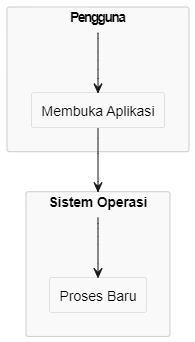
\includegraphics[width=0.4\textwidth]{asset/user process creation.png}
    \caption{Pengguna menciptakan proses baru ketika membuka aplikasi.}
\end{figure}


Pengguna adalah entitas langsung yang memulai proses ketika berinteraksi dengan perangkat lunak. Setiap aplikasi yang dijalankan pengguna akan mengarah pada pembuatan proses baru yang membutuhkan manajemen sumber daya oleh sistem operasi.

\paragraph{Sistem Operasi sebagai Pencipta Proses}

Sistem operasi juga bertindak sebagai pencipta proses, terutama untuk proses-proses latar belakang yang diperlukan untuk menjaga komputer berjalan dengan baik. Proses-proses ini sering kali tidak terlihat oleh pengguna tetapi tetap penting untuk fungsionalitas dasar sistem.

\begin{itemize}
    \item  Sistem operasi menciptakan proses-proses yang menjalankan tugas penting seperti pengelolaan jaringan, penjadwalan tugas, dan pengelolaan file. Tugas-tugas ini dilakukan tanpa memerlukan interaksi langsung dari pengguna.
    \item  Beberapa proses latar belakang, yang dikenal sebagai daemon, selalu berjalan untuk menangani tugas-tugas seperti pengelolaan memori atau pengaturan koneksi jaringan.
    \item  Sistem operasi secara otomatis menangani kapan proses-proses ini dibuat, diatur, dan diakhiri, berdasarkan kebutuhan sistem dan kondisi saat ini.
\end{itemize}

\begin{figure}[h]
    \centering
    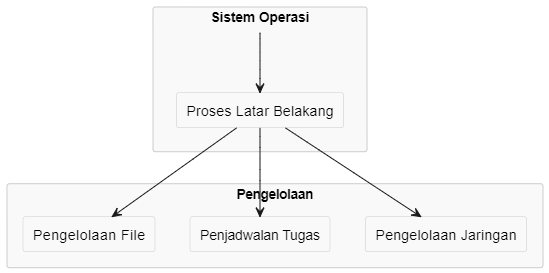
\includegraphics[width=0.9\textwidth]{asset/os background process creation.png}
    \caption{Pengguna menciptakan proses baru ketika membuka aplikasi.}
\end{figure}

Proses yang diciptakan oleh sistem operasi tidak membutuhkan interaksi pengguna secara langsung, namun sangat penting untuk menjaga stabilitas dan efisiensi komputer. Contoh dari proses-proses ini termasuk manajemen memori, keamanan sistem, dan pengelolaan perangkat keras.

\paragraph{Proses Lain sebagai Pencipta Proses (Parent-Child Relationship)}

Selain pengguna dan sistem operasi, sebuah proses juga dapat menciptakan proses lain, yang dikenal sebagai \textit{spawning}. Dalam sistem operasi, sebuah proses induk (\textit{parent process}) dapat menciptakan proses anak (\textit{child process}) untuk menjalankan tugas-tugas tertentu secara paralel atau terpisah.

\begin{itemize}
    \item \textit{Proses Parent-Child} Ketika proses induk menciptakan proses anak keduanya dapat berjalan secara bersamaan. Proses anak dapat mewarisi sebagian besar sumber daya dari proses induk, namun tetap dapat berjalan secara independen.
    \item \textit{Pembuatan Sub-Proses} Proses induk mungkin menciptakan sub-proses untuk menjalankan bagian-bagian spesifik dari suatu program, misalnya, dalam pengelolaan tab di browser web.
    \item \textbf{Contoh :} Google Chrome membuat proses terpisah untuk setiap tab yang dibuka oleh pengguna. Setiap tab berfungsi sebagai proses anak dari proses utama Chrome, yang mengelola seluruh operasi aplikasi.
\end{itemize}

\begin{figure}[h]
    \centering
    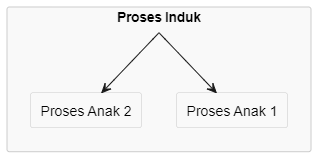
\includegraphics[width=0.7\textwidth]{asset/parent child process creation.png}
    \caption{Pengguna menciptakan proses baru ketika membuka aplikasi.}
\end{figure}


Penciptaan proses oleh proses lain memungkinkan multitasking dan pembagian beban kerja dalam sistem operasi. Ini penting dalam aplikasi yang membutuhkan banyak tugas secara bersamaan tanpa mengganggu tugas utama.

\paragraph{Scheduler sebagai Pengelola Proses}
Meskipun bukan entitas yang secara langsung menciptakan proses, scheduler dalam sistem operasi memainkan peran penting dalam mengelola proses yang sedang berjalan. Scheduler bertanggung jawab untuk mengalokasikan waktu CPU ke setiap proses yang sedang berjalan berdasarkan prioritas dan kebutuhan.

\begin{itemize}
    \item \textit{Pembagian Waktu CPU} Scheduler memastikan bahwa setiap proses mendapatkan giliran yang adil untuk menggunakan CPU, terutama ketika banyak proses berjalan bersamaan.
    \item \textit{Manajemen Prioritas} Proses dengan prioritas lebih tinggi seperti proses sistem, dapat diberikan waktu CPU lebih sering dibandingkan proses dengan prioritas lebih rendah, seperti aplikasi yang tidak aktif.
    \item \textit{Pengelolaan Multitasking} Dengan bantuan scheduler sistem operasi dapat menjalankan banyak aplikasi secara bersamaan tanpa menurunkan performa keseluruhan.
\end{itemize}

\begin{figure}[h]
    \centering
    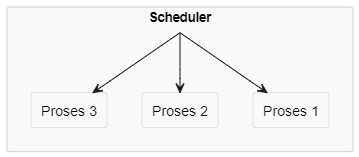
\includegraphics[width=0.9\textwidth]{asset/scheduler cpu allocation.png}
    \caption{Pengguna menciptakan proses baru ketika membuka aplikasi.}
\end{figure}

Meskipun scheduler tidak menciptakan proses, ia berperan penting dalam pengelolaan proses, memastikan bahwa semua proses berjalan dengan efisien dan sistem tetap responsif terhadap tugas-tugas pengguna.

\subsubsection{Proses \textit{Termination}}
\begin{itemize}
    \item Definisi Proses \textit{Termination}
     (isi materi disini)

    \item Jenis-jenis \textit{Termination}
    (Isi materi disini)

    \item Apa yang Terjadi Setelah \textit{Termination}
    (isi materi disini)
\end{itemize}

\begin{thebibliography}{99}

    \bibitem{silberschatz2018} 
    Silberschatz, A., Galvin, P. B., \& Gagne, G. (2018). \textit{Operating System Concepts} (10th ed.). Wiley.

\bibitem{stallings2017} 
    Stallings, W. (2017). \textit{Operating Systems: Internals and Design Principles} (9th ed.). Pearson.
\end{thebibliography}

\subsection{Introduction to Threads}
This section introduces the concept of threads and their relation to processes, covering:
\begin{itemize}
    \item Single-threaded vs. multi-threaded processes
    \item Benefits of multithreading
\end{itemize}

\begin{figure}[h]
    \centering
    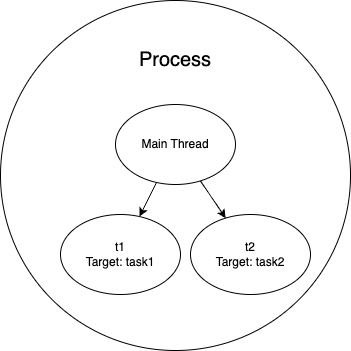
\includegraphics[width=0.5\textwidth]{D:/Tugas/Sisop/os_report_mid2024/a_class/asset/example.png} % Sesuaikan nama file dan ukurannya
    \caption{Ini adalah gambar contoh dari multithreading.}
    \label{fig:contoh_gambar}
\end{figure}


Seperti yang terlihat pada Gambar \ref{fig:contoh_gambar}, inilah cara menambahkan gambar dengan keterangan.

\subsection{File Systems}
File systems provide a way for the operating system to store, retrieve, and manage data. This section explains:
\begin{itemize}
    \item File system structure
    \item File access methods
    \item Directory management
\end{itemize}

\subsection{Input and Output Management}
Input and output management is key for handling the interaction between the system and external devices. This section includes:
\begin{itemize}
    \item Device drivers
    \item I/O scheduling
\end{itemize}

\subsection{Deadlock Introduction and Prevention}
Explores the concept of deadlocks and methods for preventing them:
\begin{itemize}
    \item Deadlock conditions
    \item Deadlock prevention techniques
\end{itemize}

\subsection{User Interface Management}
This section discusses the role of the operating system in managing the user interface. Topics covered include:
\begin{itemize}
    \item Graphical User Interface (GUI)
    \item Command-Line Interface (CLI)
    \item Interaction between the user and the operating system
\end{itemize}

\subsection{Virtualization in Operating Systems}
Virtualization allows multiple operating systems to run concurrently on a single physical machine. This section explores:
\begin{itemize}
    \item Concept of virtualization
    \item Hypervisors and their types
    \item Benefits of virtualization in modern computing
\end{itemize}

\section{Assignments and Practical Work}
\subsection{Assignment 1: Process Scheduling}
Students were tasked with implementing various process scheduling algorithms (e.g., FCFS, SJN, and RR) and comparing their performance under different conditions.
\subsubsection{Group 1}
\begin{python}
    class Process:
    def __init__(self, pid, arrival_time, burst_time):
        self.pid = pid
        self.arrival_time = arrival_time
        self.burst_time = burst_time
        self.completion_time = 0
        self.turnaround_time = 0
        self.waiting_time = 0
\end{python}

\begin{table}[htbp] % Optional: For floating position
    \centering
    \begin{tabular}{|c|c|c|} % Defines number of columns and alignment (c = center, l = left, r = right). '|' creates vertical lines.
    \hline
    Header 1 & Header 2 & Header 3 \\ % Column headers
    \hline
    Row 1, Column 1 & Row 1, Column 2 & Row 1, Column 3 \\ % First row of data
    \hline
    Row 2, Column 1 & Row 2, Column 2 & Row 2, Column 3 \\ % Second row of data
    \hline
    \end{tabular}
    \caption{Your table caption} % Optional: For adding a caption
    \label{tab:your_label} % Optional: For cross-referencing the table
\end{table}
\subsection{Assignment 2: Deadlock Handling}
In this assignment, students were asked to simulate different deadlock scenarios and explore various prevention methods.

\subsection{Assignment 3: Multithreading and Amdahl's Law}
This assignment involved designing a multithreading scenario to solve a computationally intensive problem. Students then applied \textbf{Amdahl's Law} to calculate the theoretical speedup of the program as the number of threads increased.
\subsubsection{Group 6}

Ragilnata, seorang mahasiswa berkulit gelap yang suka bercanda, sedang duduk di ruang lab sambil liat instagram, ketika dosennya Pak Abdul tiba-tiba memberi tugas mendadak tentang multithreading. "Eh Ragilnata, udah saatnya kamu ngerjain tugas daripada liat mirai terus," kata Pak Abdul sambil marah.

Ragilnata diminta untuk membuat program yang memproses data gambar berukuran besar untuk mendeteksi objek tertentu (misalnya pisang). Karena gambar-gambar ini lumayan besar dan berat secara komputasi, Ragilnata memutuskan untuk menggunakan multithreading biar cepat selesai, soalnya dia gak mau ngerjain ini sendirian semalaman.

Total waktu untuk menyelesaikan proses deteksi objek tanpa multithreading adalah 10 detik. Dari seluruh proses, sekitar 70\% dari total eksekusi bisa diparalelkan, sedangkan sisanya harus tetap dieksekusi secara serial karena constraint dari algoritma deteksi objeknya.

Dengan informasi ini, Ragilnata pun mencoba menghitung berapa kecepatan (speedup) yang bisa dicapai berdasarkan \textbf{Amdahl’s Law} jika ia menggunakan 4 thread. Sebelum mulai koding, Ragilnata jadi mikir-mikir, "Kira-kira pake 4 thread aja gak sih? Atau cukup pake 2 doang biar hemat resource?"

\textbf{Pertanyaan:}
\begin{enumerate}
    \item Hitung berapa speedup (S) yang bisa Ragilnata capai jika dia menggunakan 4 thread.
    \item Apakah hasil speedup tersebut signifikan dibandingkan dengan jika Ragilnata hanya menggunakan 2 thread? Hitung juga speedup untuk 2 thread dan bandingkan hasilnya.
    \item Menurut kamu, berapa jumlah thread yang sebaiknya digunakan oleh Ragilnata, dan kenapa?
\end{enumerate}

\textbf{Jawaban:}

\begin{enumerate}
    \item \textbf{Speedup dengan 4 thread} \\
    Amdahl's Law:
        \[
        S = \frac{1}{(1 - P) + \frac{P}{N}}
        \]
        Di mana:

        $P$ = proporsi bagian yang bisa diparalelkan = 0.7 \\
        $N$ = jumlah thread = 4

        \textbf{Hasil perhitungan menggunakan Python}

    \begin{python}
        # Definisikan variabel
        P = 0.7
        N = 4
            
        # Fungsi untuk menghitung speedup berdasarkan Amdahl's Law
         def amdahl_speedup(P, N):
            return 1 / ((1 - P) + (P / N))
            
        # Hitung speedup
        speedup = amdahl_speedup(P, N)
        speedup

        #Hasil : 2.1052631578947367
           
    \end{python}
    Jadi, speedup dengan 4 thread adalah sekitar \textbf{2.105 kali} lebih cepat.
    
    \item \textbf{Speedup dengan 2 thread} \\
    \begin{python}
        # Update jumlah thread menjadi 2
        N = 2

        # Hitung speedup dengan 2 thread
        speedup_with_2_threads = amdahl_speedup(P, N)
        speedup_with_2_threads

        #Hasil : 1.5384615384615383
    \end{python}
    Jadi, speedup dengan 2 thread adalah sekitar \textbf{1.538 kali} lebih cepat. \\
    Speedup dengan 4 thread (2.105) lebih signifikan dibandingkan dengan 2 thread (1.538). Artinya, menggunakan 4 thread lebih efisien dalam hal kecepatan.
    
    \item \textbf{Jumlah thread optimal} \\
    Jumlah thread bergantung pada resource yang tersedia. Jika Ragilnata punya resource yang cukup (seperti CPU dengan core yang banyak), maka menggunakan 4 thread lebih baik karena speedup-nya lebih signifikan. Namun, jika resource terbatas, 2 thread juga sudah memberikan peningkatan yang lumayan tanpa membebani sistem.
\end{enumerate}

\subsection{Assignment 4: Simple Command-Line Interface (CLI) for User Interface Management}
Students were tasked with creating a simple **CLI** for user interface management. The CLI should support basic commands such as file manipulation (creating, listing, and deleting files), process management, and system status reporting.

\subsection{Assignment 5: File System Access}
In this assignment, students implemented file system access routines, including:
\begin{itemize}
    \item File creation and deletion
    \item Reading from and writing to files
    \item Navigating directories and managing file permissions
\end{itemize}

\section{Conclusion}
The first half of the course introduced core operating system concepts, including process management, scheduling, multithreading, and file system access. These topics provided a foundation for more advanced topics to be covered in the second half of the course.

\end{document}